	\documentclass[11pt, a4paper, spanish]{article}

\usepackage{alltt}

%%%%%%%%%% COMIENZO DEL PREAMBULO %%%%%%%%%%

%Info sobre este documento
\author{Mart\'n Cammi}
\title{Trabajo Pr\'actico de Algoritmos y Estucturas de datos III}

%\usepackage{infostyle}                                                  % provee un look & feel similar a un documento Word
\usepackage[top=2.5cm, bottom=2.5cm, left=2.5cm, right=2.5cm]{geometry}  % m\'argenes
\usepackage[ansinew]{inputenc}                                           % permite que los acentos del estilo \'a\'e\'i\'o\'u salgan joya
\usepackage[spanish, activeacute]{babel}                                 % idioma espaniol, acentos f\'aciles y deletreo de palabras
\usepackage{indentfirst}                                                 % permite indentar un parrafo a mano
\usepackage{caratula}                                                    % incluye caratula est\'andar
\usepackage{graphicx}                                                    % permite insertar gr\'aficos
\usepackage{color}                                                       % permite el uso de colores en el documento
\usepackage{amssymb}
\usepackage[pdfcreator={TexLive!, LaTeX2e con TeXnicCenter},
			pdfauthor={Grupo: "1"},
			pdftitle={Algoritmos III - Trabajo Pr\'actico 2},
			pdfsubject={Trabajo Pr\'actico 1},
			pdfkeywords={Prismas, Esferas, Punto de corte, puente, pizza},
			pdfstartview=FitH,            % Fits the width of the page to the window
			bookmarksnumbered,            % los bookmarks numerados se ven mejor...
			colorlinks,                   % links con bellos colores
			linkcolor=magenta]            % permite cambiar el color de los links
			{hyperref}                    % Permite jugar con algunas cosas que aparecer\'an en el PDF final

%RESTAURAR

\usepackage{algorithm}							% Permite tabular un codigo
\usepackage{algorithmic}
%\floatname{algorithm}{Algoritmo}
\renewcommand{\listalgorithmname}{Lista de algoritmos}
\renewcommand{\algorithmicrequire}{\textbf{Entrada:}}
\renewcommand{\algorithmicensure}{\textbf{Salida:}}
\renewcommand{\algorithmicend}{\textbf{fin}}
\renewcommand{\algorithmicif}{\textbf{si}}
\renewcommand{\algorithmicthen}{\textbf{entonces}}
\renewcommand{\algorithmicelse}{\textbf{si no}}
\renewcommand{\algorithmicelsif}{\algorithmicelse,\ \algorithmicif}
\renewcommand{\algorithmicendif}{\algorithmicend\ \algorithmicif}
\renewcommand{\algorithmicfor}{\textbf{para}}
\renewcommand{\algorithmicforall}{\textbf{para todo}}
\renewcommand{\algorithmicdo}{\textbf{hacer}}
\renewcommand{\algorithmicendfor}{\algorithmicend\ \algorithmicfor}
\renewcommand{\algorithmicwhile}{\textbf{mientras}}
\renewcommand{\algorithmicendwhile}{\algorithmicend\ \algorithmicwhile}
\renewcommand{\algorithmicloop}{\textbf{repetir}}
\renewcommand{\algorithmicendloop}{\algorithmicend\ \algorithmicloop}
\renewcommand{\algorithmicrepeat}{\textbf{repetir}}
\renewcommand{\algorithmicuntil}{\textbf{hasta que}}
\renewcommand{\algorithmicprint}{\textbf{imprimir}} 
\renewcommand{\algorithmicreturn}{\textbf{devolver}} 
\renewcommand{\algorithmictrue}{\textbf{cierto }} 
\renewcommand{\algorithmicfalse}{\textbf{falso }} 
 % mi archivo de traducci\'on			

%\selectlanguage{spanish}

%\selectlanguage{spanish}
\linespread{1.3}                    % interlineado equivalente al 1.5 l\'ineas de Word...
\pagestyle{myheadings}              %encabezado personalizable con \markboth{}{}
\markboth{}{Algoritmos III  - Trabajo Pr\'actico 2 - Cammi, Garbi, Kretschmayer}
\headsep = 30pt                     % separaci\'on entre encabezado y comienzo del p\'arrafo

%\addtolength{\oddsidemargin}{-2cm}	% configuracion IDEAL!!!
%\addtolength{\textwidth}{4cm}
%\addtolength{\textheight}{2cm}

% macro 'todo' para To-Do's
\def\todo#1{\textcolor{red}{#1}}

% Macro 'borde' para un texto con borde
\newsavebox{\fmbox}
\newenvironment{borde}[1]
{\begin{lrbox}{\fmbox}\begin{minipage}{#1}}
{\end{minipage}\end{lrbox}\fbox{\usebox{\fmbox}}\\[10pt]}

%%%%%%%%%% FIN DEL PREAMBULO %%%%%%%%%%

\begin{document}

\materia{Algoritmos y Estucturas de datos III}
\submateria{Segundo Cuatrimestre de 2011}
\titulo{Trabajo Pr\'actico 2}
\subtitulo{Problema1: Esferas vs Prismas. \ \ \ \ \ \ \ \ \ \ \ \ \ \ \ \ \ \ \ \ \ \ \ \ \ \ \ \ \ \ \ \ \ \ \  Problema2: Puntos de corte y puentes. \ \ \ \ \ \ \ \ \ \ \ \ \ \ \ \ \ \ Problema3: M\'as Pizza entre amigos.}
\grupo{Grupo: `1'}
\integrante{Cammi, Mart\'in}{676/02}{martincammi@gmail.com}
\integrante{Garbi, Sebasti\'an}{179/05}{garbyseba@gmail.com}
\integrante{Kretschmayer, Daniel}{310/99}{daniak@gmail.com}

\maketitle

\thispagestyle{empty}

\tableofcontents

\newpage


\textbf{Ejecuci\'on del TP}
\label{sec:ejecucion}

	\subsection{Lenguaje utilizado}
		
		El lenguaje utilizado para el trabajo pr\'actico ha sido \emph{Java}, compilando con la versi\'on 1.5 de la Virtual Machine.
		
		El trabajo se acompa\~{n}a con los fuentes de la soluci\'on que puede importarse en IDE de Eclipse o ejecutarse desde l\'inea de comandos.

	\subsection{Como ejecutar el TP}
	
	\textbf{\underline{Desde l\'inea de comandos}}
	\begin{itemize}
			\item{Posicionarse en el directorio Algo3Tp2}
			\item{Copiar all\'i el archivo de entrada para el problema i, por ejemplo Ej1.in}
			\item{Ejecutar el comando: \emph{java -cp ./bin problema1.Ej1}}
	\end{itemize}
	Esto generar\'a el archivo Ej1.out con la soluci\'on en el mismo directorio Algo3Tp2.

	\textbf{\underline{Desde el Eclipse}}
	
	Primero importaremos el proyecto:	
	
	\begin{itemize}
			\item{Seleccionar File $\Rightarrow$ Import.}
			\item{Seleccionar General $\Rightarrow$ Existing Projects into Workspace $\Rightarrow$ Next.}
			\item{Seleccionar el directorio llamado Algo3Tp2.}
			\item{Finish.}
	\end{itemize}
	
	Desde la vista de \textbf{Package Explorer} bajo el paquete \textbf{src} aparecer\'an tres paquetes m�s y dentro de cada uno de ellos los siguientes archivos de java:\\

	\begin{center}
		%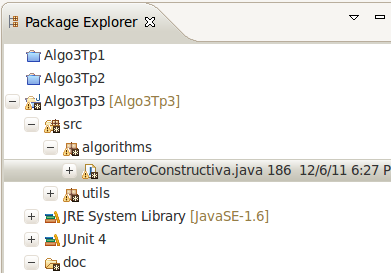
\includegraphics[scale=0.65]{others/packageExplorer.png}\\
		COLOCAR IMAGEN CORRECTA
	\end{center}

\newpage

	Para ejecutar un problema:

	\begin{itemize}
			\item{Posicionarse en el directorio Algo3Tp2}
			\item{Copiar en el directorio Algo3Tp2 el archivo de entrada para el problema i, por ejemplo Ej1.in}
			\item{Con bot\'on derecho Run As $\Rightarrow$ Java Application. Se ejecutar\'a el problema seleccionado.}
	\end{itemize}
	Esto generar\'a el archivo Ej1.out con la soluci\'on en el mismo directorio Algo3Tp2.

\newpage

% Conviene poner las secciones como diferentes archivos,
% sobre todo cuando se trabaja en equipo.
% Es m\'as f\'acil para sincronizar mediante control de versiones.
%\input{Introducci\'on}

% Problema1
\section{Problema1: Esferas vs Prismas}
\label{sec:problema1}
	\subsection{Introducci\'on}

	La guerra contra los prismas se ha declarado y debemos ayudar a las esferas a ganarla.\\
	La batalla se libra en un campo minado de prismas, agrupados uno al lado del otro en forma de una grilla de $l x a$. Cada prisma tienen una altura y un rango y una esfera puede destruir un prisma golpe\'andolo en la cabeza y continuar destruyendo otros prismas si estos est\'an contiguos y tienen menor altura que el que ya destruy'o. El nivel de destrucci\'on es la suma de todos los rangos de los prismas ca\'idos en combate.\\
	 Nuestro objetivo es idear un algoritmo para que las esferas puedan producir la mayor cantidad de destrucci\'on posible.\\
	
	\subsection{Explicaci\'on de la soluci\'on}
	
	El objetivo es lograr encontrar un camino que parta desde un prisma y vaya recorriendo prismas adyacentes de menor altura y que este camino tenga el rango o nivel de destrucci\'on m\'aximo posible.

	La idea del algoritmo es recorrer estos caminos al rev\'es. Comenzaremos recorriendo cada prisma de la grilla y para cada uno de ellos haremos recursi'on preguntando si pudo haber venido de alg\'un otro mayor, preguntando a sus 4 vecinos. Si alguno de ellos es mayor que \'el significa que un camino de destrucci\'on pudo haber venido de ese prisma y volveremos recursivamente a preguntarle a ese prisma de donde pudo haber venido. De esta manera iremos recorriendo los prismas hasta que encontremos un prisma mayor a todos sus vecinos y no podamos continuar. Este prisma ser\'a el caso base, es decir el prisma el inicial para uno de los caminos que pueda tomar la esfera. 

A medida que vamos recorriendo estos caminos en la recursi\'on iremos al mismo tiempo calculando el \emph{Nivel de Destrucci\'on} y en base a \'el guardaremos para cada prisma un \emph{de donde vino} para poder luego identificar el camino de mayor destrucci\'on.

En el siguiente ejemplo se muestra el recorrido del algoritmo, supondemos para simplificar este ejemplo que el rango de cada prisma es igual a su altura, as\'i el prisma de altura 1 tiene un rango igual a 1.

	\begin{center}
		\includegraphics[scale=0.40]{p1/PrismasyEsferas1.png}\\
	\end{center}

En el ejemplo figuran 4 prismas, comenzaremos calculando la mayor destrucci\'on del el prisma 1.

	\begin{center}
		\includegraphics[scale=0.40]{p1/PrismasyEsferas2.png}\\
	\end{center}

Los prismas de mayor altura adyacentes al prisma 1 son dos, el que est\'a a su derecha y el que est\'a abajo. El algoritmo recorrer\'a a sus vecinos en sentido de las agujas del reloj comenzando por el vecino superior. En este caso el Prisma 1 no tiene vecino superior por lo que continuar\'a por su vecino de la derecha.

	\begin{center}
		\includegraphics[scale=0.40]{p1/PrismasyEsferas3.png}\\
	\end{center}

Ahora situados en el prisma 2, recorreremos todos los vecinos con altura mayor que \'el, el \'unico es el prisma 3. (el gui\'on indica de que prisma se vino desde la recursi\'on)

	\begin{center}
		\includegraphics[scale=0.40]{p1/PrismasyEsferas4.png}\\
	\end{center}

Hemos llegado al prisma 3 el cual no tiene vecinos mayores que \'el con lo cual formar\'a el inicio de un camino de destrucci\'on.

	\begin{center}
		\includegraphics[scale=0.40]{p1/PrismasyEsferas5.png}\\
	\end{center}

Le asignamos el rango del mismo prisma que es tres (lo indicaremos en la parte inferior derecha de cada prisma) ya que no pudo haber venido de otro prisma.

	\begin{center}
		\includegraphics[scale=0.40]{p1/PrismasyEsferas6.png}\\
	\end{center}

Retornamos entonces en la recursi\'on volviendo al prisma 2 y preguntamos si la destrucci\'on acumulada de 2 supera la de su vecino reci\'en calculado 3. Como 2 todav\'ia no tiene asignado destrucci\'on acumulada lo actualizaremos con la de 3 mas el valor de su rango, es decir 5.


	\begin{center}
		\includegraphics[scale=0.40]{p1/PrismasyEsferas6-5.png}\\
	\end{center}

Retornamos entonces en la recursi\'on volviendo al prisma 1 y preguntamos si la destrucci\'on acumulada de 1 supera la de su vecino reci\'en calculado 2. Como 1 todav\'ia no tiene asignado destrucci\'on acumulada lo actualizaremos con la de 2 mas el valor de su rango, es decir 6.\\

	\begin{center}
		\includegraphics[scale=0.40]{p1/PrismasyEsferas7.png}\\
	\end{center}

Al mismo tiempo hemos retornado en la recursi\'on de 1 habiendo obtenido el valor de destrucci\'on de su vecino derecho, nos falta ver el nivel de destrucci\'on de su vecino de abajo.

	\begin{center}
		\includegraphics[scale=0.40]{p1/PrismasyEsferas8.png}\\
	\end{center}

Ahora situados en el prisma 2 (de abajo), recorreremos todos los vecinos con altura mayor que \'el, el \'unico es el prisma 3 nuevamente. 

	\begin{center}
		\includegraphics[scale=0.40]{p1/PrismasyEsferas9.png}\\
	\end{center}

Como de iteraciones anteriores el prisma 3 ya tiene calculado su nivel de destrucci\'on, no entraremos en recursi\'on para el prisma 3 nuevamente, sino que simplemente preguntamos si la destrucci\'on acumulada de 2 supera la de su vecino 3 ya calculado. Como 2 todav\'ia no tiene asignado destrucci\'on acumulada lo actualizaremos con la de 3 mas el valor de su rango, es decir 5.

	\begin{center}
		\includegraphics[scale=0.40]{p1/PrismasyEsferas10.png}\\
	\end{center}

Finalmente hemos vuelto de la recursi\'on del prisma 1 y ya no quedan vecinos por recorrer.
Sin embargo pueden haber quedado prismas sin visitar que no hayan sido alcanzables desde la recursi\'on del prisma 1. Es por eso que asi como hicimos con el prisma 1 recorreremos todos los prismas de la grilla para asegurarnos que no quede ninguno sin visitar pero con la salvedad de que no entraremos en la recursi\'on en ellos si su nivel de destrucci\'on ya fue calculado por alg�n otro camino previo. Esto nos evitar\'a hacer recursi\'on innecesariamente.\\

En el ejemplo, como ya para todos los prismas se han logrado calcular sus niveles de destrucci\'on, si bien los recorreremos para verificarlo no haremos recursi\'on en ninguno de ellos nuevamente.


Cabe aclarar que para poder calcular el camino final debemos guardar un par de datos.\\
Cada vez que actualizamos el nivel de destrucci\'on de un prisma, guardamos tambi\'en el vecino del cual obtuvo mayor nivel para luego poder identificar el camino de mayor destrucci\'on. Tambi\'en guardamos el prisma que haya acumulado el mayor nivel para luego comenzar de \'el a reconstruir el camino.

	\begin{center}
		\includegraphics[scale=0.40]{p1/PrismasyEsferas11.png}\\
	\end{center}

En el ejemplo el prisma que acumul\'o mayor destrucci\'on fue el 1 con un nivel de 6. El 1 obtuvo parte de ese nivel de parte del prisma 2 de su derecha (se guard\'o que venia del 2). El prisma 2 a su vez qued\'o con un nivel de 5 y obtuvo parte de \'el del prisma 3 (se guard\'o que venia del 3).
El prisma 3 obtuvo su nivel de \'el mismo, ya que sus vecinos tenian todos altura menor con lo cual se guard\'o que venia de \'el mismo (Esto nos ayudar\'a al rearmar el camino saber cuando terminar de recorrer, es decir, cuando un prisma haya venido de si mismo.\\

El mayor camino de destrucci\'on entonces con un nivel de 6 ser\'a:\\

	\begin{center}
		\includegraphics[scale=0.40]{p1/PrismasyEsferas12.png}\\
	\end{center}

El algoritmo trabaja realizando una mezcla entre backtracking volviendo recursivamente para obtener la mejor soluci\'on y programaci\'on din\'amica por la cual una vez calculado el nivel de un prisma lo guarda en una variable de acceso constante para no realizar c\'alculos innecesarios.

\newpage
	
\subsection{Pseudo-c\'odigo}

\begin{algorithm}
\caption{calcularCaminoDeMaximaDestruccion}
\label{alg1}
\begin{algorithmic}

	\FOR {Cada prisma de la matriz}
		\IF {tiene guardado el nivel de destrucci\'on acumulado}
			\RETURN nivel de destrucci\'on acumulado del prisma
		\ELSE
			\FOR {Cada vecino de mayor altura}
				\STATE calcularMaximaDestruccion(vecino)
			\ENDFOR				
			vecinoConMaximaDestrucci\'on = calcular cual de los anteriores es el vecino de m\'axima destrucci\'on

			\IF {prisma.destruccionAcumulada > vecinoConMaximaDestrucci\'on.destrucci\'onAcumulada}
				\STATE prisma.destrucci\'onAcumulada = prisma.rango
				\STATE prisma.desdeDondeVino = prisma.INICIO
			\ELSE
				\STATE prisma.destrucci\'onAcumulada = prisma.rango + vecinoConMaximaDestrucci\'on.destrucci\'onAcumulada
				\STATE prisma.desdeDondeVino = vecinoConMaximaDestrucci\'on
			\ENDIF
		\ENDIF

		\IF{vecinoConMaximaDestrucci\'on > maximo}
			\STATE maximo = vecinoConMaximaDestrucci\'on
		\ENDIF
	\ENDFOR

	\WHILE {!maximo.desdeDondeVino != prisma.INICIo}
		\STATE agrego el prisma a una lista para luego devolverla
	\ENDWHILE
	 
\end{algorithmic}
\end{algorithm}	


\subsection{Modelo Elegido}

	El modelo elegido ser\'a el \emph{Modelo Uniforme} porque las operaciones son escencialmente comparaciones y sumas que podemos asumir de orden constante sin que por ello afecte la complejidad del algoritmo.
\newpage
	
\subsection{Complejidad}

	El algoritmo tendr\'a que recorrer todos los elemento de la grilla por lo menos una vez esto da un orden de $O(l \cdot a)$.\\

	Por otro lado tenemos que tener en cuenta las llamadas recursivas, habr\'a una por cada vez que un prisma visite a otro prisma superior a \'el (recordemos que el algoritmo busca los caminos de forma inversa). 

	\begin{center}
		\includegraphics[scale=0.30]{p1/PrismasyEsferasUnidasPorAristas.png}\\
	\end{center}

Los prismas est\'an agrupados en una grilla y se recorren a trav\'es de alguno de sus posibles cuatro vecinos adyacentes. Podemos imaginarnos dicha grilla como un grafo en donde cada arista representa un pasaje recursivo de un prima a uno de mayor altura. Por la forma de recorrer del algoritmo pasaremos una sola vez por cada una de estas ``aristas`` ya que en caso de tener el nivel precalculado no deberemos hacer recursi\'on.\\

De esta forma para cada prisma el algoritmo tendr\'a como posibilidades para recursi\'on todas las fechas salientes. En el ejemplo anterior las flechas corresponden a recursiones reales sobre los prismas. En cualquier grilla el \'unico caso en que una de estas aristas no sea recorrida es que ambos prismas tengan la misma altura. En cualquier otro caso o bien un prisma vecino a otro lo llamar\'a en una recursi\'on o bien su vecino lo llamar\'a a el.

	\begin{center}
		\includegraphics[scale=0.30]{p1/PrismasyEsferasUnidasPorAristasDetalle.png}\\
	\end{center}

En el peor de los casos entonces el algoritmo har\'a una cantidad de llamadas recursivas que equivale a la cantidad aristas del supuesto grafo y esto suceder\'a si ning\'un prisma adyacente a otro tiene la misma altura. La cantidad de aristas de este grafo es la cantidad de aristas que hay de largo $(l-1)$ por la altura que es $a$ para las aristas horizontales m\'as la cantidad de aristas que hay de alto $(a-1)$ por el largo $l$, lo que en total da:

\begin{center}
 $(l-1) \cdot a + (a-1) \cdot l$
\end{center}

Por \'ultimo debemos calcular el camino de m\'axima destrucci\'on esto se logra partiendo del nodo de m\'aximo nivel calculado y yendo hacia atr\'as hasta el nodo de mayor altura, esto tomar\'a $(l \cdot a)$ ya que en el peor caso este camino podr\'ia incluir a todos los prismas.

De esta manera el orden final queda:

\begin{center}
		$O( (l \cdot a) + (l-1) \cdot a + (a-1) \cdot l + (l \cdot a))$
\end{center}
\begin{center}
		$O( 2 \cdot (l \cdot a) + (l-1) \cdot a + (a-1) \cdot l)$
\end{center}
\begin{center}
		$O( 2 \cdot (l \cdot a) + (l \cdot a) - l + (l \cdot a) - a)$
\end{center}
\begin{center}
		$O( 4 \cdot (l \cdot a) - l - a)$
\end{center}
\begin{center}
y finalmente este orden pertenece a:\\
		$O( l \cdot a)$
\end{center}


Ahora bien, para describir la complejidad en funci\'on del tama\~{n}o de la entrada debemos tener en cuenta la representaci\'on del n\'umero de entrada n en la computadora.
	Un n\'umero n ser\'a representado como $\log n$ bits.\\
	
	Definimos entonces el tama\~{n}o de entrada como:
	
	\begin{center}
 	$T$ = log(a) + log( l) + $\displaystyle\sum_{i=0}^{l*a}(h_{i}+r_{i})$\\
	\end{center}
	
	Donde $h_{i}$ es la altura y $r_{i}$ es el rango del elemento i en la grilla. Si quitamos la sumatoria del lado derecho, T pasar\'a a ser m\'as grande que el miembro derecho pues $\displaystyle\sum_{i=0}^{l*a}(h_{i}+r_{i}) >= 0$
	
	\begin{center}
	$T => log(a) + log(l)$
	\end{center}
	O similarmente:

	\begin{center}
	$log(a) + log(l) <= T$
	\end{center}
	Por propiedad de logaritmos:

	\begin{center}
	$log(a \cdot l) <= T$
	\end{center}
	Aplico ${2}^{x}$ a ambos lados:

	\begin{center}
	$a \cdot l <= {2}^{T}$
	\end{center}
	
	Finalmente entonces la complejidad temporal en base a T es exponencial del orden de:

	\begin{center}
	 $O(2^{T})$
	\end{center}

\newpage


\newpage

\subsection{Tests}


	\textbf{Mejor caso: }
		Una grilla en la que todos los prismas tengan la misma altura ser\'a el mejor caso, porque s\'olamente recorreremos toda la grilla con total de $l \cdot a$ m\'as $1$ por la complejidad de calcular el camino de mayor da\~{n}o que s\'olamente incluir\'a un \'unico prisma.\\

\begin{center}
   \centering \includegraphics[scale=0.30]{p1/PrismasyEsferasMejorCaso.png}
   \verb$        $
   \centering \includegraphics[scale=0.30]{p1/PrismasyEsferasMejorCasoSolucion.png}
\end{center}

A la izquierda la grilla de prismas enojados y a la derecha el camino de mayor destrucci\'on formado s\'olo por el prisma de altura 1.\\

	\textbf{Caso promedio y Cuasi-peor caso: }
		Ser\'an los casos en que el algoritmo logre hacer la mayor cantidad de recursiones (recorrer todas las ``aristas`` ficticias) pero que la soluci\'on final no incluya en su camino a todos los prismas. Este es un caso promedio tambi\'en porque lo m\'as probable que suceda asumiento una distribuci\'on normal de las alturas de los prismas es que prismas adyacentes tengan alturas diferentes y favorezcan la recursi\'on.
En el ejemplo siguiente se marca con aristas las recursiones realizadas de un prisma para con otro y en negrita las que terminar\'an formando la soluci\'on del problema.

\begin{center}
   \centering \includegraphics[scale=0.30]{p1/PrismasyEsferasCuasiPeorCaso.png}
   \verb$        $
   \centering \includegraphics[scale=0.30]{p1/PrismasyEsferasCuasiPeorCasoSolucion.png}
\end{center}

	
	\textbf{Peor caso: }
		Este caso se dar\'a cuando a semejanza del anterior logren recorrerse todas ``aristas`` ficticias y al mismo tiempo el camino de mayor destrucci\'on sea total, es decir incluya a todos los prismas.
	
\begin{center}
   \centering \includegraphics[scale=0.30]{p1/PrismasyEsferasPeorCasoSolucion.png}
\end{center}	

\subsection{Gr\'aficos}

	Mediciones de los tests en modelo uniforme

\subsection{Conclusiones}

\newpage

% Problema2
\section{Problema2: Puntos de corte y Puentes}
\label{sec:problema2}
	\subsection{Introducci\'on}
	
	\subsection{Explicaci\'on de la soluci\'on}
	
\newpage
	
\subsection{Pseudo-c\'odigo}
	
\begin{algorithm}
\caption{Puntos de corte y Puentes}
\label{alg1}
\begin{algorithmic}

	\STATE	Colocar aqui el algoritmo...
	 
\end{algorithmic}
\end{algorithm}	

\subsection{Modelo Elegido}

\newpage
	
\subsection{Complejidad}
	
\begin{algorithmic}
	
	\STATE	Colocar aqui el algoritmo...
			
\end{algorithmic}	

\newpage


\newpage

\subsection{Tests}
	
\subsection{Gr\'aficos}

\subsection{Conclusiones}

\newpage


% Problema3
\section{Problema3: M\'as pizza con amigos}
\label{sec:problema3}
	\subsection{Introducci\'on}
	Se quiere pedir una pizza extra gigante para un grupo de amigos. Cada uno de los amigos puede tener a lo sumo 2 preferencias de elementos que quiere que est\'en o no en la pizza.
	Como no se puede satisfacer todas las preferencias de cada uno de los amigos, se pretende buscar una soluci\'on donde al menos una de las preferencias de cada amigo sea satisfecha, o responder que no es posible.
	\subsection{Explicaci\'on de la soluci\'on}
	Antes de explicar la soluci\'on elegida, comentaremos algunas decisiones tomadas ad hoc:
	\begin{itemize}

		\item En la entrada puede llegar a venir en las preferencias de alguno de los comensales un ingrediente repetido. Se descartaran las apariciones repetidas de ese ingrediete en caso que la decisi\'on tomada sobre el mismo sea la misma EJ: +A+A lo tomaremos como +A.
		Si alguna de las repeticiones tiene la desici\'on contraria (EJ: +A-A), entonces asumiremos que este comensal est\'a satisfecho por defecto y no ser\'a procesado, ya que cualquier decisi\'on tomada sobre el ingrediente en cuesti\'on lo satisfacer\'a.
		
		\item Otro caso ad hoc es cuando en la entrada viene una linea vacia (solo ';'), en este caso asumiremos que no existe una pizza que satisfaga al menos una preferencia de este comensal ya que este no tiene preferencias.
		
		\item Por \'ultimo, en los casos que tenemos al menos un comensal, los iremos agregando en una lista de comensales insatisfechos ordenados por cantidad de preferencias, de mayor a menor. Por ejemplo, si el comensal 1 tiene una preferencia, y el comensal 2 y 3 tiene dos, agregaremos a la lista primero al comensal 2 y 3, y luego al primer comensal. 
		
	\end{itemize}
	La idea del algoritmo es la siguiente: Nosotros siempre tendremos comensales con 1 o 2 preferencias.
	Tenemos una lista de todos los comensales insatisfechos, y en las primeras posiciones de \'esta, est\'an todos los comensales con dos preferencias (si es que los hay), y luego los dem\'as comensales con 1 preferencia (tambi\'en, si los hay). Empezaremos recorriendo los comensales de atr\'as hacia adelante (lo hicimos as\'i para poder sacarlos de la lista en orden constante). Por lo tanto, primero calculamos los comensales a los que debemos satisfacerle la preferencia si o si (los que tengan 1 sola preferencia).
	Lo que haremos para cada comensal es:
	
	\begin{itemize}
	
	\item Si tiene una sola preferencia, la forzamos a que se cumpla (ya que se debe cumplir siempre una preferencia de cada comensal), agregamos esa preferencia como soluci\'on parcial del algoritmo y luego, realizaremos la validaci\'on 1, que explicamos a continuaci\'on. Supongamos que tengo el comensal con la preferencia +A.\\
	
	\textbf{Validaci\'on 1:} Con esta preferencia (+A en el ejemplo), chequeamos en el resto de los comensales insatisfechos, si esta preferencia hace cumplir alguna de sus preferencias tambi\'en, y de ser a\'i, sacamos a ese comensal de los comensales insatisfechos (ya que una de sus preferencias fue satisfecha). En el ejemplo, si otro comensal tiene entre sus preferencias a +A, ya cumple que una de sus preferencias fue satisfecha.
	En cambio, si ese comensal tiene la preferencia opuesta (-A en el ejemplo), puede pasar 2 cosas: 
	
		\begin{itemize}
		
		\item Si tiene una sola preferencia, no tendr\'a soluci\'on, ya que no podr\'e satisfacer ese pedido (no podr\'e satisfacer a 2 comensales, uno con +A y otro con -A). 
		
		\item En cambio, si el comensal tiene 2 preferencias, debemos formar a la preferencia que no es la opuesta a la que estabamos calculando. Siguiendo el ejemplo, si el comensal tiene -A+B, entonces debo forzar que pase +B, agregando el +B como soluci\'on parcial, quitando a este comensal de la lista de comensales insatisfechos y repetir la validaci\'on 1 para el ingrediente +B.
		
		\end{itemize}
		
		Si todos los comensales quedan satisfechos, entonces devuelvo la soluci\'on, caso contrario, tomo el pr\'oximo comensal de la lista de insatisfechos.
				
		\item En cambio, si el comensal tiene 2 preferencias (ya seguro habr\'e calculado a todos los comensales con una sola, si los hab\'ia), entonces fuerzo la primera preferencia para que suceda, agrego la preferencia como soluci\'on parcial, saco al comensal de la lista de comensales y realizo la validaci\'on 1 con el ingrediente (por ejemplo, +A). Si luego de sacar a todos los comensales con la validaci\'on, me quedan todos satisfechos, entonces devuelvo la soluci\'on, caso contrario, tomo el pr\'oximo comensal de la lista de insatisfechos. Si pude satisfacer a todos forzando la primer preferencia, devuelvo la soluc\'on y el algoritmo termina con esa soluci\'on.
		En cambio, si no pude llegar a una soluci\'on forzando la primer preferencia (ten\'ia 2), entonces debo realizar los mismos pasos que cuando forzamos la primer preferencia, pero ahora con la segunda.
		
		El algoritmo termina cuando todos los comensales quedan satisfechos, o bien cuando no se podr\'a satisfacer a alg\'un comensal (que retorna que no es posible).\\
		
		\textbf {Ejemplo pr\'actico:}
		Para verlo con un ejemplo sencillo, vamos con un ejemplo pr\'actico: Si en el archivo de entrada me vienen 5 comensales con las siguientes preferencias, para n=5 (n es cantidad de ingredientes):\\
		\textbf{Comensal 1}(+A)\\ 
		\textbf{Comensal 2}(+A+B)\\
		\textbf{Comensal 3}(+D -C)\\
		\textbf{Comensal 4}(+D +E)\\
		\textbf{Comensal 5}(-A +E).\\
		
		Al leer el archivo, se agrega al comensal con una sola preferencia al final de la lista (el comensal 1, con +A). Entonces, al ejecutar el algoritmo, agrega a la soluci\'on parcial la preferencia +A y fuerza que esto suceda. Chequea entre los otros comensales si hay alguna que tenga +A (en este caso, el comensal 2) y lo saca de la lista de insatisfechos.
		Tambi\'en chequea si hay un comensal con la preferencia opuesta, y en este caso el comensal 5 tiene -A, por lo que debe forzar +E para que satisfaga alguna de sus preferencias, y agrega el +E a la soluci\'on parcial, y realiza nuevamente la validaci\'on con el +E a ver si satisface a otro comensal. En este caso, el comensal 4 se satisface con el +E, por lo que lo saca de la lista de insatisfechos, y ya no tiene m\'as comensales que sacar con esta validaci\'on, por lo que itera al pr\'oximo comensal insatisfecho (en este caso, me queda uno solo, el comensal 3), por lo que, siguiendo el algoritmo, tomar\'a la primer preferencia (el +D) y retornar\'a la pizza ABCDE.
		
	 \end{itemize}
	
	\subsection{Pseudo-c\'odigo}
	\begin{algorithmic}
	%Para mas referencia ver http://en.wikibooks.org/wiki/LaTeX/Algorithms_and_Pseudocode
	
	\STATE funcion resolver()
	\STATE listaComensalesInsatisfechos $\gets$ todosComensales
	\STATE listaIngredientesChequear $\gets$ listaVacia
	\STATE pizzaTieneSolucion $\gets$ \TRUE
	\STATE solucionParcial $\gets$ vacioString
	\WHILE {!listaComensalesInsatisfechos.isEmpty() y pizzaTieneSolucion}
		\STATE ultComensal $\gets$ listaComensales.size() - 1; 
		\STATE preferenciaForzada $\gets$ preferencia1DelComensal
		\IF {Se puedeAgregarASolucionParcial(preferenciaForzada)}
			\STATE listaIngredientesChequear.add(preferenciaforzada)
			\STATE	listaComensalesInsatisfechos.remove(ultComensal)			
			\STATE solucionParcial $\gets$ solucionParcial + preferenciaForzada
		\ELSE
			\STATE solucionParcial $\gets$ No Es Posible
			\STATE pizzaTieneSolucion $\gets$ \FALSE
		\ENDIF
		
		\WHILE {!listaIngredientesChequear.isEmpty() y !listaComensalesInsatisfechos.isEmpty()\\ y pizzaTieneSolucion}
			\FOR {j = listaComensales.size() - 1 hasta j = 0}
					\IF {preferencia1DelComensalJ = Preferencia(listaIngredientesChequear.get(0)) o  \\
							 preferencia2DelComensalJ = Preferencia(listaIngredientesChequear.get(0))}
					\STATE listaComensalesInsatisfechos.remove(ultComensal)    /*ya esta satisfecho*/
				\ELSE
					\IF {preferencia1DelComensalJ = preferenciaOpuesta(listaIngredientesChequear.get(0)) o
							 preferencia2DelComensalJ = preferenciaOpuesta(listaIngredientesChequear.get(0))}
						\IF {ComensalJTieneUnaSolaPreferencia}
							\STATE solucionParcial $\gets$ No Es Posible
							\STATE pizzaTieneSolucion $\gets$ \FALSE
						\ELSE
							\STATE solucionParcial $\gets$ solucionParcial + OtraPreferenciaNoEsLaOpuesta
							\STATE listaIngredientesChequear.add(OtraPreferenciaNoEsLaOpuesta)
							\STATE listaComensalesInsatisfechos.remove(j)
						\ENDIF
					\ENDIF
				\ENDIF
			\ENDFOR
		\ENDWHILE
	\ENDWHILE 
	
	\end{algorithmic}		\subsection{Modelo Elejido}
	
	Para calcular la complejidad de este algoritmo utilizaremos el modelo $Uniforme$, ya que por mas que la cantidad de datos de la entrada crezca, las operaciones sobre cada uno de ellos es constante y podemos asumirla en $O(1)$
	\subsection{Complejidad}
	$n$ = Cantidad de Ingredientes\\
	$m$ = Cantidad de Comensales\\
	$prefs$ = Nro Total de preferencias\\
	Preguntar si un comensal prefiere un ingrediente es $O(1)$\\
	Preguntar si quedan comensales insatisfechos es $O(1)$\\
	Mover un comensal de una lista a otra es $O(1)$\\
		
	El algoritmo, realiza para cada comensal (m veces) si puede o no agregar la preferencia a la soluci\'on parcial, agrega esa preferencia a una lista de preferencias a chequear en O(1), y vuelve a iterar por todos los comensales que a\'un quedan insatisfechos con esta preferencia a chequear si se satisface para los dem\'as comensales. A lo sumo, chequear\'a los otros m-1 comensales, que son los que est\'an insatisfechos en la primera iteraci\'on. Entonces, en el peor caso, para los m comensales validar\'a si puede o o agregar a los otros m-1. Pero si no llega a una soluci\'on con el primer ingrediente, realiza exactamente el mismo algoritmo para la segunda preferencia.
	
	Entonces, en el peor caso, lo que puede pasar es que, tenga un algoritmo que deba recorrer la lista el orden del algoritmo es $O(2*m^{2})$
	
	Esto deja el algoritmo en una complejidad te\'orica de $O(m^{2})$\\
	
	Las preferencias pueden estar dispersas de maneras variadas entre los comensales, ya que pueden haber muchos comensales con 1 o 2 preferencias cada uno.
	En este caso, $prefs$ $\geq$ $m$ ya que no tiene sentido tener comensales sin preferencias porque el algoritmo terminar\'ia ni bien se termina de leer la entrada. \\
	Por otra parte necesitamos una cota inferior para $T$; Sabemos que el ingrediente mas chico tiene tama�o de entrada $1$ asi que se cumple $T \geq \sum_{i = 1}^{prefs}{1} = prefs$.\\
	Teniendo en cuenta estas observaciones, sabemos que $T$ $\geq$ $prefs$ $\geq$ $m$, luego como la complejidad del algoritmo es $O(m^{2})$ concluimos que la complejidad del algoritmo con respecto al tama�o de la entrada pertenece a $O(T^{2})$.
	
	\subsection{Tests}
	\textbf{Tipo1:} El algoritmo tiene bien marcado cuales vendr\'an a ser sus mejores casos. A los ya triviales, como que venga un comensal vac\'io o que hayan 2 comensales con preferencias opuestas (que devuelven que no es posible), vamos a concentrarnos en los que al menos recorren una vez todos los comensales, que son los que pueden llegar a dar una soluci\'on posible.
	Realizando varios tests, pudimos notar que en el mejor caso, el algoritmo puede ser lineal en la cantidad de comensales, ya que en la primera iteraci\'on, por ejemplo, puede tomar un ingrediente (el +A en el ejemplo), y luego recorrer\'a a todos los dem\'as comensales preguntando si el +A los satisface, que en el ejemplo es cierto. 
	
	A estos los llamaremos $Tipo 1$\\
	Ej.
	\begin{verbatim}
	8
	+A+B;
	+A+C;
	+A+D;
	+A+E;
	+A+F;
	+A+G;
	+A+H;
	.
	\end{verbatim}
	\textbf{Tipo2:}	Con respecto al peor caso, nos pusimos a analizar lo que cre\'iaamos, ser\'an los 2 posibles peores casos, donde en cada iteraci\'on se satisfaga a un solo comensal. En el ejemplo, en la primera iteraci\'on se sacar\'a el comensal 1 (+A), en la segunda el comensal 2 (+B) y as\'i sucesivamente.
	\begin{verbatim}
	8
	+A+B;
	+B+C;
	+C+D;
	+D+E;
	+E+F;
	+F+G;
	+G+H;
	.
	\end{verbatim}
	\textbf{Tipo3:} El pr\'oximo caso que analizamos, es el tener el primer comensal con una cierta preferencia (-F en este caso), y debe chequear todos los comensales (porque es el \'ultimo de la lista de comensales insatisfechos) hasta darse cuenta que hay otro con +F (preferencia opuesta) que lo fuerza a elegir la preferencia +A). Luego, en la pr\'oxima iteraci\'on sucede lo mismo con el +B, que lo fuerza al tener el +C y as\'i sucsivamente. En cada iteraci\'on saca 1 solo comensal, y este esta a lo \'ultimo de la lista de comensales insatisfechos.
	\begin{verbatim}
	8
	-F+G;
	-E-D;
	+E-D;
	+D-C;
	+C-B;
	-A+B;
	+A+F;
	.
	\end{verbatim}
	\textbf{Tipo4:} No contentos con las mediciones obtenidas notamos que, por mas que el $Tipo 3$ parec\'ia el peor caso, pod\'ia haber un caso peor a\'un, que es cuando realiza algo similar que el anterior, pero llega a un momento que forzando ingredientes, no puede llegar a una soluci\'on y debe realizar nuevamente todos los c\'alculos, pero con el Ingrediente 2 del comensal 1. Primero toma el comensal 1 con el -F, y en la primera iteraci\'on, tiene 2 comensales con la preferencia opuesta, y debe forzar el -E y el +A (comensales 5 y 6). Cuando calcula todos los comensales que se satisfacen con -E, termina forzando ingredientes hasta llegar a forzar -A (comensal 2). Termina de calcular las preferencias forzadas, y luego calcula el comensal 7, que tiene la preferencia +A para hacer cumplir, lo que hace que la soluci\'on no sea posible, y deba rehacer todo el algoritmo, pero esta vez forzando la preferencia 2 del comensal 1. La estructura es:
	\begin{verbatim}
	8
	-F+G;
	-A+B;
	+C-B;
	+D-C;
	+E-D;
	-E+F;
	+A+F;
	.
	\end{verbatim}
	\subsection{Gr\'aficos}
	%grafico tipo 1
	%grafico tipo 2
	%grafico tipo 3
	%grafico tipo 4
	
	Explicaci\'on del gr\'afico de $Tipo 1$
	En este gr\'afico, se puede ver el mejor caso propuesto, donde el orden de complejidad es lineal a la cantidad de comensales. Esto tiene sentido, ya que todos comparten la misma preferencia, y en la primera iteraci\'on ya sacamos a todos de la lista de insatisfechos.
	
	\begin{center}
		\includegraphics[scale=0.65]{p2/MedicionesTipo1.png}
	\end{center}
	
	
	Explicaci\'on del gr\'afico de $Tipo 2$
	Aca, podemos ver que los valores se acercan mucho al orden que planteamos, ya que en cada iteraci\'on solo sacamos de a un comensal, pero como termina siempre calculando con el primer ingrediente de todos, no se acerca tanto a la par\'abola te\'orica del orden de complejidad como quer\'iamos.
	
		\begin{center}
			\includegraphics[scale=0.65]{p2/MedicionesTipo2.png}
		\end{center}
	
	Explicaci\'on del gr\'afico de $Tipo 3$
	Los valores se acercan m\'as a\'un al orden que expusimos, tambi\'en sacamos solo de a un comensal por iteraci\'on, pero como ya no solo agarra el primer ingrediente, sino que debe ir forzando ingredientes en cada iteraci\'on, los ordenes de complejidad son mayores a los del $Tipo 2$.
	
		\begin{center}
			\includegraphics[scale=0.65]{p2/MedicionesTipo3.png}
		\end{center}
	
	Explicaci\'on del gr\'afico de $Tipo 4$
	Aca planteamos el peor caso del alg\'oritmo, donde en la primer iteraci\'on, me quedan 2 comensales con la preferencia opuesta, por lo que debo forzar una preferencia. Al forzar la primera de los 2, puedo sacar a todos los comensales de los satisfechos menos a 1, y cuando quiero satisfacer a este \'ultimo, veo que no puedo satisfacerlo, por lo que debo realizar todo el algoritmo de nuevo, para la preferencia 2 del comensal 1. 
	
		\begin{center}
			\includegraphics[scale=0.65]{p2/MedicionesTipo4.png}
		\end{center}
	
	\subsection{Conclusiones}
	Luego de estudiar bastante el problema, vemos que el algoritmo se comporta bastante similar a lo que esperabamos. Hay un mejor caso lineal, que es cuando todos los comensales coinciden en una preferencia, y por otro lado, pudimos notar que hay varios casos pat\'ol\'ogicos, pero que los ordenes de complejidad no difieren demasiado entre s�, que son muy similares al del $O(m^{2})$.
	Los ordenes de complejidad mejoraron al ordenar la lista de comensales por cantidad de preferencias (primero calculo los que tienen 1 preferencia), ya que si en la entrada, nos ven\'ian comensales con ua solo ingrediente, esto nos permit\'ia forzar ingredientes y poder encontrar m\'as facilmente las entradas en donde las pizzas no eran posibles.\\ 
	Por otro lado, notamos que, si vienen muchos comensales como entrada del algoritmo, el orden de complejidad no era cuadr\'atico (el te\'orico), sino que era menor. Esto se debe ya que hay solo 26 posibles ingredientes posibles y en caso de haber m\'as de 26 comensales, seguro los ingredientes de ellos se repiten y el algoritmo no se comporta tan mal como con menos cantidad de comensales.
	
	
	
\newpage

\end{document}
